\documentclass[preprint, 3p, authoryear]{elsarticle} %review=doublespace preprint=single 5p=2 column
%%% Begin My package additions %%%%%%%%%%%%%%%%%%%

\usepackage[hyphens]{url}

  \journal{Journal of Marine Systems} % Sets Journal name

\usepackage{lineno} % add
  \linenumbers % turns line numbering on

\usepackage{graphicx}
%%%%%%%%%%%%%%%% end my additions to header

\usepackage[T1]{fontenc}
\usepackage{lmodern}
\usepackage{amssymb,amsmath}
\usepackage{ifxetex,ifluatex}
\usepackage{fixltx2e} % provides \textsubscript
% use upquote if available, for straight quotes in verbatim environments
\IfFileExists{upquote.sty}{\usepackage{upquote}}{}
\ifnum 0\ifxetex 1\fi\ifluatex 1\fi=0 % if pdftex
  \usepackage[utf8]{inputenc}
\else % if luatex or xelatex
  \usepackage{fontspec}
  \ifxetex
    \usepackage{xltxtra,xunicode}
  \fi
  \defaultfontfeatures{Mapping=tex-text,Scale=MatchLowercase}
  \newcommand{\euro}{€}
\fi
% use microtype if available
\IfFileExists{microtype.sty}{\usepackage{microtype}}{}

\ifxetex
  \usepackage[setpagesize=false, % page size defined by xetex
              unicode=false, % unicode breaks when used with xetex
              xetex]{hyperref}
\else
  \usepackage[unicode=true]{hyperref}
\fi
\hypersetup{breaklinks=true,
            bookmarks=true,
            pdfauthor={},
            pdftitle={Migratory species influence seabird biomass},
            colorlinks=false,
            urlcolor=blue,
            linkcolor=magenta,
            pdfborder={0 0 0}}

\setcounter{secnumdepth}{5}
% Pandoc toggle for numbering sections (defaults to be off)


% tightlist command for lists without linebreak
\providecommand{\tightlist}{%
  \setlength{\itemsep}{0pt}\setlength{\parskip}{0pt}}

% From pandoc table feature
\usepackage{longtable,booktabs,array}
\usepackage{calc} % for calculating minipage widths
% Correct order of tables after \paragraph or \subparagraph
\usepackage{etoolbox}
\makeatletter
\patchcmd\longtable{\par}{\if@noskipsec\mbox{}\fi\par}{}{}
\makeatother
% Allow footnotes in longtable head/foot
\IfFileExists{footnotehyper.sty}{\usepackage{footnotehyper}}{\usepackage{footnote}}
\makesavenoteenv{longtable}

% Pandoc citation processing
\newlength{\cslhangindent}
\setlength{\cslhangindent}{1.5em}
\newlength{\csllabelwidth}
\setlength{\csllabelwidth}{3em}
\newlength{\cslentryspacingunit} % times entry-spacing
\setlength{\cslentryspacingunit}{\parskip}
% for Pandoc 2.8 to 2.10.1
\newenvironment{cslreferences}%
  {}%
  {\par}
% For Pandoc 2.11+
\newenvironment{CSLReferences}[2] % #1 hanging-ident, #2 entry spacing
 {% don't indent paragraphs
  \setlength{\parindent}{0pt}
  % turn on hanging indent if param 1 is 1
  \ifodd #1
  \let\oldpar\par
  \def\par{\hangindent=\cslhangindent\oldpar}
  \fi
  % set entry spacing
  \setlength{\parskip}{#2\cslentryspacingunit}
 }%
 {}
\usepackage{calc}
\newcommand{\CSLBlock}[1]{#1\hfill\break}
\newcommand{\CSLLeftMargin}[1]{\parbox[t]{\csllabelwidth}{#1}}
\newcommand{\CSLRightInline}[1]{\parbox[t]{\linewidth - \csllabelwidth}{#1}\break}
\newcommand{\CSLIndent}[1]{\hspace{\cslhangindent}#1}

\usepackage{setspace}\doublespacing
\usepackage{pdflscape}
\DeclareUnicodeCharacter{0394}{\ensuremath{\Delta}}
\newcommand{\blandscape}{\begin{landscape}}
\newcommand{\elandscape}{\end{landscape}}
\usepackage{booktabs}
\usepackage{longtable}
\usepackage{array}
\usepackage{multirow}
\usepackage{wrapfig}
\usepackage{float}
\usepackage{colortbl}
\usepackage{pdflscape}
\usepackage{tabu}
\usepackage{threeparttable}
\usepackage{threeparttablex}
\usepackage[normalem]{ulem}
\usepackage{makecell}
\usepackage{xcolor}



\begin{document}


\begin{frontmatter}

  \title{Migratory species strongly affect seabird biomass in seasonal assemblages off northeast Aotearoa/New Zealand}
  
    \author[MarSci-Otago,MatStat-Otago]{Nicholas W. Daudt%
  \corref{cor1}%
  }
   \ead{nicholaswdaudt@gmail.com} 
   
    \author[MarSci-Otago,FarOut]{Marta Guerra%
  %
  }
    \author[NIWA,FarOut]{Tom Brough%
  %
  }
    \author[DOC,FarOut]{Sarah L. Dwyer%
  %
  }
    \author[FarOut]{Jochen R. Zaeschmar%
  %
  }
    \author[MatStat-Otago]{Matthew R. Schofield%
  %
  }
    \author[MarSci-Otago]{Robert O. Smith%
  %
  }
    \author[FURG]{Leandro Bugoni%
  %
  }
    \author[ASG]{Eric J. Woehler%
  %
  }
    \author[MarSci-Otago]{William J. Rayment%
  %
  }
  
    \affiliation[MarSci-Otago]{Department of Marine Science, University of Otago, Dunedin, Aotearoa New Zealand}
    \affiliation[MatStat-Otago]{Department of Mathematics and Statistics, University of Otago, Dunedin, Aotearoa New Zealand}
    \affiliation[FarOut]{Far Out Ocean Research Collective, Paihia, Aotearoa New Zealand}
    \affiliation[NIWA]{National Institute of Water and Atmospheric Research, Dunedin, Aotearoa New Zealand}
    \affiliation[DOC]{Department of Conservation, Aotea Great Barrier Island, Aotearoa New Zealand}
    \affiliation[FURG]{Institute of Biological Sciences, Universidade Federal do Rio Grande -- FURG, Rio Grande, RS, Brazil}
    \affiliation[ASG]{Australasian Seabird Group, BirdLife Australia, Hobart, Australia}
    \cortext[cor1]{Corresponding author}
  
  \begin{abstract}
  
   Migratory species may influence structural components of species assemblages, such as biomass and diversity patterns. A total of 10 ship-based, strip-transect seabird surveys were undertaken in all seasons (2019--2024) off the northeast coast of Northland, Aotearoa/New Zealand. Almost all seabird species recorded were migratory or wide-ranging dispersive (23 of 25). Multivariate model-based ordinations revealed that season primarily explained species assemblages, while including environmental variables such as sea surface temperature and chlorophyll-\emph{a} (useful proxies for studying seabird distribution) offered little extra explanatory power at the assemblage level. There was no clear spatial pattern in the assemblages, suggesting that the study area was used uniformly by the species present at the time. The total seabird biomass present was strongly influenced by the seasonal occurrence of four medium-sized, migratory procellariiforms: t\={a}iko (black petrel), rako (Buller’s shearwater), \={o}i (grey-faced petrel) and toanui (flesh-footed shearwater). The biomass estimates showed an eight-fold increase from winter (243 kg/km$^2$) to summer (1885 kg/km$^2$). Northland will likely be the first region in Aotearoa/New Zealand to experience the consequences of oceanic warming. The study establishes a baseline against which to measure potential future changes in seabird occurrences. Based on descriptive and modelling approaches, the study demonstrated the role of species' phenologies in shaping assemblages of seabird species and their impact on total estimated biomass, which may affect ecosystem functioning and energy fluxes.
  \end{abstract}
  
  \begin{keyword}
    At-sea surveys \sep Biomass \sep Community ecology \sep Ecosystem functioning \sep Migratory species \sep Phenology \sep Seabird assemblages
  \end{keyword}
  
 \end{frontmatter}

\hypertarget{highlights}{%
\section*{Highlights}\label{highlights}}
\addcontentsline{toc}{section}{Highlights}

\begin{itemize}
\item
  First quantitative data on seabird assemblages off northeast Aotearoa/New Zealand
\item
  Composition of oceanic seabird assemblages were primarily explained by season
\item
  Approximate eight-fold increase in seabird biomass from winter to summer
\item  
  High numbers of migratory and wide-ranging dispersive species were recorded throughout the year
\item
  Four medium-sized procellariforms characterised seasonal assemblages
\end{itemize}

\newpage

\section{Introduction}

Understanding species' distributions is essential for their conservation and management. At large temporal (yearly or longer) and spatial (global) scales, occurrence and distribution patterns of species are mostly well documented. However, this is often not the case at finer scales (seasonal/regional) \citep{ferrier2002}. The current gaps in our knowledge largely derive from geographically significant gaps in particular areas \citep{miloslavich2011, hughes2021}, precluding a holistic understanding of global biodiversity patterns \citep{sastre2009} and our ability to describe the relationships among species and their environments. Further, the scarcity of baseline distributional data in many regions prevents the prediction of impacts of environmental changes on species and communities due to climate fluctuations and/or anthropogenic stressors. Baseline studies are thus paramount to establishing benchmarks for monitoring environmental changes and their subsequent consequences on biota.

One approach to monitor biodiversity is using surrogates or proxies, such as species assemblages \citep{rodrigues2007}. Assemblages are groups of species sharing space and time \citep{stroud2015}. As they experience similar environmental conditions and pressures, they can be used in biodiversity assessments \citep{ferrier2002, rodrigues2007}. It has been shown that assemblages in both terrestrial and marine environments are changing on decadal time-scales in response to climate change \citep{dornelas2014, antao2022}. These changes are mainly associated with species tracking their preferred environmental niches \citep{chen2011, pinsky2019, lenoir2020}. Marine taxa appear to be tracking environmental changes faster than terrestrial taxa \citep{pinsky2019, antao2020, lenoir2020}. Identifying changes in marine species assemblages (i.e., changes in their structure) may provide early signals arising from changes in marine environments.

Structural components of communities, including diversity (e.g.,~richness, turnover, dominance), nutrient dispersion, energy flux and ecosystem services \citep{magurran2010, bauer2014, kurasawa2024}, have all been shown to vary according to season. The magnitude of migratory and seasonal movements of wide-ranging species has been particularly important when describing these structural changes in communities \citep{bauer2014, schlagel2020}. For example, marine megafauna, such as seabirds, are responsible for seasonally influencing estimated prey consumption in ecosystems and nutrient, carbon and nitrogen cycling at sea and on land \citep{woehler1997, wing2014, doughty2016, steibl2024}. Therefore, seasons can play a crucial role in biodiversity patterns and ecosystem functioning and should be incorporated in descriptions of ecological patterns \citep{forrest2010, banks-leite2012, ponti2023}.

Seabirds are adapted to breed on land and feed at sea, exposing them to threats in both environments, such as invasive predators on land \citep{wanless2007} and bycatch at sea \citep{gianuca2017}. Consequently, many seabird populations are decreasing, leading seabirds to be recognised as the most threatened group of birds globally \citep{dias2019}. During the breeding season seabirds behave as central-place foragers, foraging at sea and returning to their nesting site between foraging trips \citep{schreiber2002book, patterson2022}. Some seabirds remain close to their colony throughout the year. After breeding, however, many species make wide-ranging dispersive flights or migrations \citep[e.g.,][]{shaffer2006, thompson2021}. These seasonal movements influence the composition and structure of oceanic seabird species assemblages \citep{hunt2014, simon2024}.

Aotearoa/New Zealand is an acknowledged global hotspot for diversity and abundance of seabirds. The country hosts the highest diversity of seabird species and number of individuals per area (densities) \citep{karpouzi2007, ramirez2017}, especially of procellariids (albatrosses and petrels) \citep{chown1998, davies2010procellariiformes}. However, the contemporary at-sea distributions of most species around Aotearoa/New Zealand remain largely unknown. In the last two decades, several species have had their distributions revealed through bio-logging \citep[e.g.,][]{shaffer2006, rayner2017, thompson2021, rayner2023}. However, these studies were mostly focused on single-species distributions, with only a few exceptions overlaying distributions of multiple species \citep[e.g.,~see][]{rayner2023}, which were mainly targeted at species breeding on the Aotearoa subantarctic islands or those breeding in the Hauraki Gulf (North Island).

Descriptions of seabird assemblages from Aotearoa/New Zealand are rare. The only published study is \citet{daudt2025}, which quantitatively detailed seabird assemblages off the Otago coast of the South Island. Other studies were qualitative, with most reporting seabird records as species accounts during brief periods or limited to one season \citep[e.g.,][]{hawke1991, odriscoll1998otago}. Using a multi-species comparative approach, \citet{vooren1972} described year-round seabird abundances in the Bay of Plenty (North Island) that are highly influenced by locally-breeding species. In light of Aotearoa/New Zealand's global importance for seabird conservation and the usefulness of assemblages to describe and monitor marine biodiversity, it is surprising that seabird assemblages in Aotearoa/New Zealand are yet to be fully described.

There are no studies describing seabird at-sea distributions off Northland \citep{mott2018} and no data from satellite-tracked species known to occur there \citep{bernard2021, carneiro2024}, despite its recognised importance for procellariiform conservation \citep{chown1998, beal2021}. Previous oceanographic studies have described the region at the macro-scale only, with sampling stations spaced \textasciitilde50 km apart and mostly to the south of Northland (see Study area, below). There is also a lack of analysis of meso- and sub-mesoscale oceanographic data in the region to support understanding observed ecological patterns \citep[but see][]{dellapenna2021}. It is notable that Northland is expected to be the first region in Aotearoa/New Zealand to show signs of tropicalisation, given it is on the margin of subtropical waters \citep{zarzyczny2024}. As marine temperatures rise as predicted, tropical species are expected to be more frequently recorded, whereas temperate species are expected to become rarer.

The area of focus in this study was off the East coast of Northland, within the rohe moana (marine tribal territory) of Ng\={a}ti Kuri, an iwi (tribe) from Northland. Ng\={a}ti Kuri are descended from the original inhabitants, the founding peoples of the northernmost peninsula of Aotearoa/New Zealand, in Te Hiku o Te Ika. Their relationship with the environment is personal and based on mutual respect and benefit. The area is of great cultural, spiritual, and ecological significance to the iwi, who have a strong interest in growing and enhancing existing m\={a}tauranga (traditional knowledge) on their rohe and its marine life. Ng\={a}ti Kuri is committed to re-visioning their ecological domains and considering the opportunities for positive change that seek to restore and protect some of the most vulnerable taonga (treasured species) and habitats remaining in Aotearoa/New Zealand. As a quantitative study focusing on the biodiversity within their rohe, this study contributes to the iwi's efforts to establish the intrinsic value of the region.

This study aimed to describe seabird assemblages off Northland, Aotearoa/New Zealand, focusing on species occurrences, relative numbers, and the seasonal dynamics of estimated biomass. As such, we provided the first quantitative assessment of seabirds in a region lacking baseline data but facing an imminent threat of tropicalisation. Seabird observations were recorded at-sea during 10 systematic, vessel-based surveys. Based on the diversity of species reported in the adjacent Hauraki Gulf \citep{gaskin2017, stateof2021} and the description of seabird assemblages elsewhere in Aotearoa/New Zealand \citep{vooren1972, brough2025, daudt2025}, a species-rich assemblage composed of several migratory and wide-ranging species was predicted for the study area. Environmental (sea surface temperature [SST] and chlorophyll-\emph{a} [CHL]) and/or temporal (season) predictors were incorporated to test whether they influenced the observed species assemblages. The presence of migratory and dispersive species was expected to strongly structure the seabird assemblage seasonally. Given that the study area has seafloor features that may influence surface conditions (submarine canyons, a large boundary current, and strong internal tide/wave activity), fine-scale associations between seabirds and local oceanography were also predicted.

% This study aimed to provide the first quantitative assessment of seabird assemblages off Northland, Aotearoa/New Zealand. Seabird observations were recorded at-sea during 10 systematic, vessel-based surveys. To investigate patterns of species occurrences, relative numbers, and biomass, a mixed approach was adopted that included spatial, descriptive, and modelling analyses. Environmental (sea surface temperature [SST] and chlorophyll-\emph{a} [CHL]) and/or temporal (season) predictors were incorporated to test whether they influenced the observed species assemblages. Based on the diversity of species reported in the adjacent Hauraki Gulf \citep{gaskin2017, stateof2021} and the description of seabird assemblages elsewhere in Aotearoa/New Zealand \citep{vooren1972, brough2025, daudt2025}, a species-rich assemblage composed of several migratory and wide-ranging species was predicted for the study area. The presence of migratory and dispersive species was expected to strongly structure the seabird assemblage seasonally. Given the study area has seafloor features that might influence surface conditions (submarine canyons, a large boundary current, and strong internal tide/wave activity), fine-scale associations between seabirds and the local oceanography were also predicted.

\section{Methods}

\subsection{Study area}

The study area is influenced by the poleward flow of the East Auckland Current (EAuC). This is a component of the broader East Australia Current (EAC) that retroflexes eastward across the Tasman Sea through a trail of eddies (the `EAC eastern extension', also called the `Tasman Front'; \citet{oke2019eac}), setting up the EAuC (Figure \ref{fig:study-area-farout}A). Starting at about 33.5\(^{\circ}\)S, the EAuC flows southeast off the northeast coast of Aotearoa/New Zealand, topographically steered by the continental shelf \citep{denham1984} and progressively becoming more offshore and weaker as it moves south towards the East Cape at 37\(^{\circ}\)S \citep{stanton1997}. Two quasi-permanent, mesoscale eddies are part of the EAuC system: the North Cape Eddy (NCE) and the East Cape Eddy (ECE) \citep[Figure \ref{fig:study-area-farout}A;][]{chiswell2015}. At its southern extent, most of the EAuC energy turns into either part of the ECE or continues into the East Cape Current (ECC), flowing southwest off the mainland until it encounters the Chatham Rise, where it is forced bathymetrically eastward (Figure \ref{fig:study-area-farout}A; \citet{stanton1997}; \citet{chiswell2015}).

\begin{figure}[H]
\centering
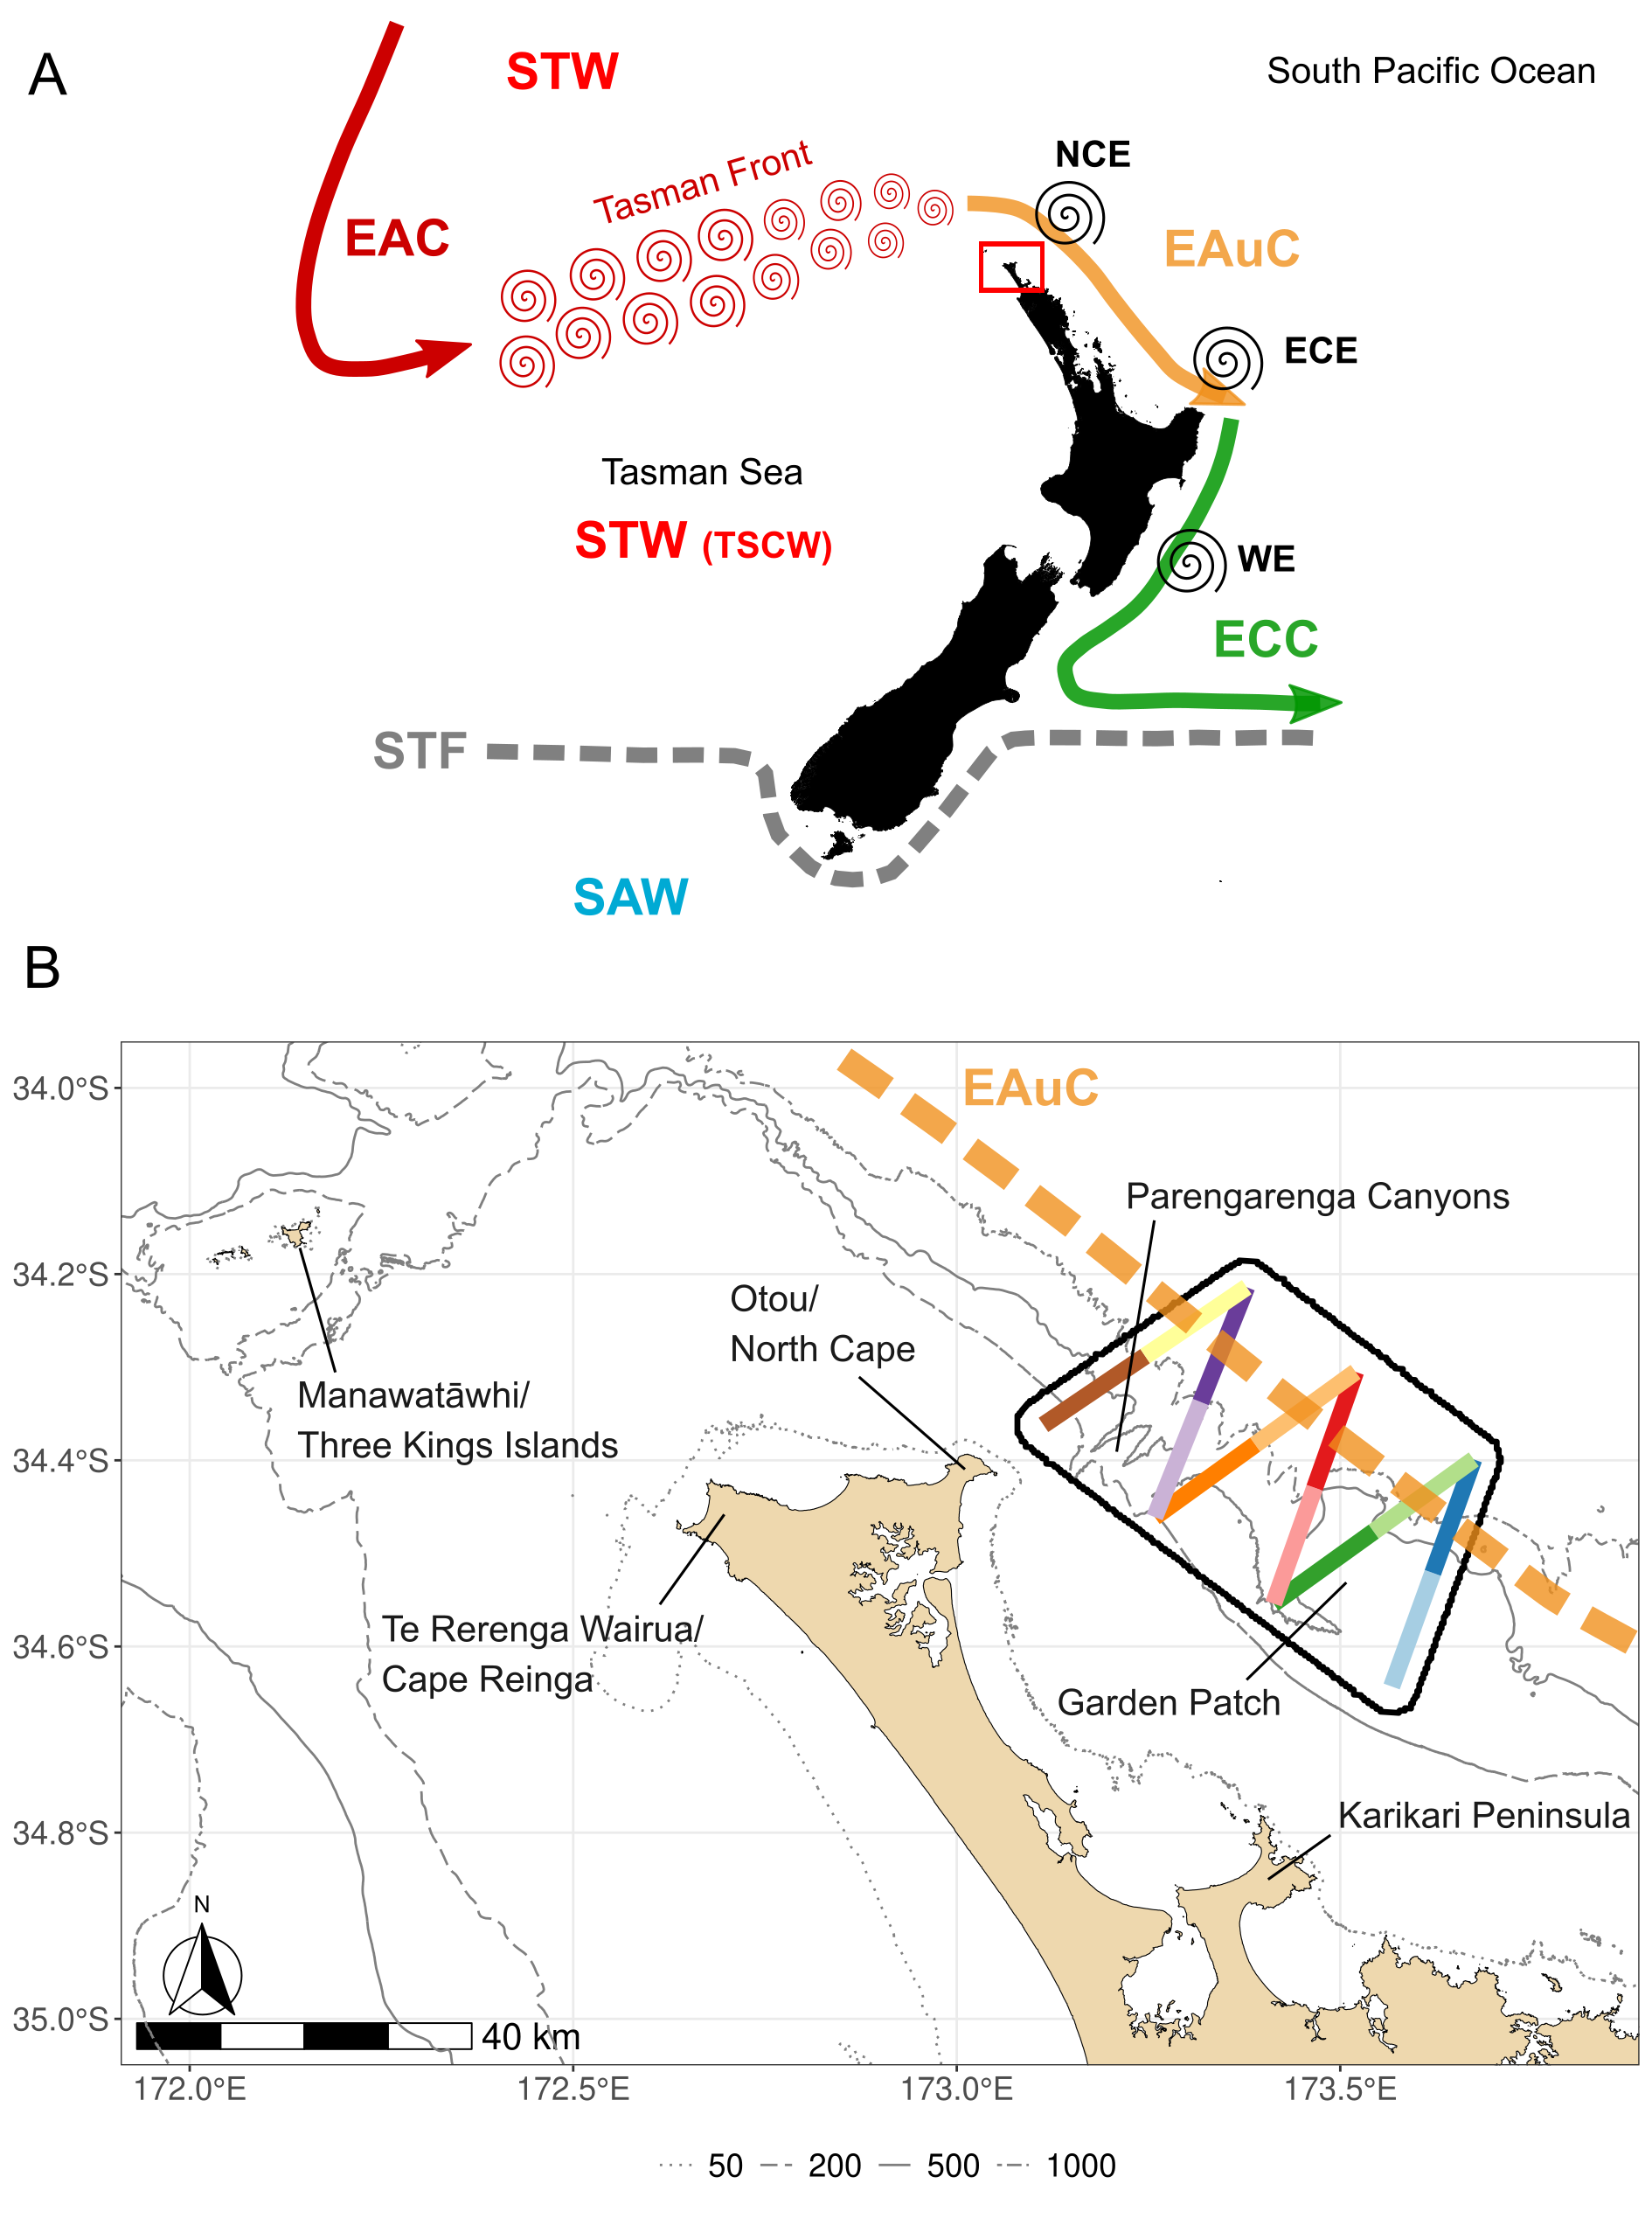
\includegraphics[width=0.73\linewidth]{study-area_far-out2.png} 
\caption[Study area, main ocean currents, and the transects where surveys were undertaken off Northland, Aotearoa/New Zealand]{Main ocean currents and processes off Aotearoa/New Zealand (A) and at the study area off Northland (B). In (A), the East Australian Current (EAC) is shown in dark red with its eastward extension (often called the 'Tasman Front'; dark red spirals) from which the East Auckland Current originates (EAuC; in orange). The EAuC extends south through the East Cape Current (ECC; in green). The three quasi-permanent eddies are shown as black spirals, the North Cape Eddy (NCE), East Cape Eddy (ECE) and Wairarapa Eddy (WE). Water masses are indicated as STW (Subtropical Water; in red), Tasman Sea Central Water (STW [TSCW]; in red) and SAW (Subantarctic Water; in blue), and the Subtropical Front (STF) is schematically represented as a grey dashed line. The red box in (A) indicates the study area in (B). In (B), the names mentioned in the text are shown for reference, and the transects where seabird counts were undertaken (and aggregated, see main text) are represented by different colours inside the black polygon, and the isobath legend is below the figure.}
\label{fig:study-area-farout}
\end{figure}

A range of meso- and sub-mesoscale oceanographic processes associated with the EAuC influence the study area \citep{dellapenna2021}. Regional fluctuations in sea surface temperatures (SST) and chlorophyll-\emph{a} (CHL) on (sub-)mesoscale time scales (\textless90 days) are associated with mesoscale eddies and linked jets that entrain cold, CHL-rich water from the areas north of Otou/North Cape. Jets of productive water flow through the region in events ranging from 10 to 90 days (Alice Della Penna and Robert O. Smith, pers. comm.). After these eddy-induced events pass through, the region returns to its usual warm, oligotrophic (low CHL) state, typical of offshore waters (i.e.,~subtropical EAC/EAuC). Dynamic events can also push coastal waters (warm, high CHL) over the shelf break into offshore waters (R. O. Smith, {pers. comm.}); however, the mechanisms of such events are yet to be described. Despite these dynamic variabilities, the study area is deemed to be stable at seasonal scales \citep{wijffels2018}.

The study area has seafloor features that possibly influence its (sub-)mesoscale oceanography: the Parengarenga Canyons and the Garden Patch (Figure \ref{fig:study-area-farout}B). The Parengarenga Canyons are three parallel canyons, rising from 500 to 200 m depth within \emph{c}. 1 km. The Garden Patch is an area characterized by several bathymetric features, including two seamounts (rising to 335 m and 505 m depth) and a bank (at about 209 m depth), with a canyon to the west that possibly provides the bank with bottom, nutrient-rich water. The latter feature is locally known to support sport fisheries for large predatory fish (e.g., various marlin [Istiophoridae] and tuna [\emph{Thunnus}] species) and commercial longlining \citep{richard2020}. Although none of these oceanographic-bathymetric interactions have been studied to date, steep seafloor features such as canyons and banks can generate localised upwellings and/or internal wave activity that generate prey concentrations attractive to foraging predators \citep{allen2001, sharples2013, sharples2021}. When cold, nutrient-rich bottom-waters encounter the seafloor they can be forced towards the surface, leading to increased primary production, which may attract marine megafauna \citep{bouchet2015, cox2018}, such as seabirds \citep{haney1987, scott2010, scott2013}.

\subsection{Data collection}

Vessel-based surveys were undertaken to document the distributions of marine megafauna off Northland. A series of six zigzag transects were designed to sample across the continental shelf slope and offshore areas, including the Garden Patch and Parengarenga Canyons (Figure \ref{fig:study-area-farout}B). At the beginning, mid- and end points of each of the six transects, the vessel stopped at stations to perform acoustic recordings (10--15 min) to assess the presence or absence of marine mammals. From the sixth voyage on, a Mang\={o}pare sensor \citep[temperature-depth recorder (TDR);][]{jakoboski2024} was cast during these stations to investigate the vertical structure of the upper 100--150 m surface water.

The surveys were undertaken aboard the ocean-going yacht SV \emph{Manawanui}, cruising under power at 7 knots (\emph{c}. 12.8 km/h). The observers' eye heights were approximately 4 m above sea level (distance to horizon \emph{c}. 7.5 km). Six to eight observers worked in pairs, rotating serially among roles every 40 minutes: marine megafauna observer (marine mammals, large fish and sharks), navigating (e.g.,~steering the vessel to stay on route), seabird observer and rest. Observers were paired (experienced with less experienced) to ensure correct species identification. At least one observer from the core group of observers (NWD, MB, TB, SLD, JRZ) was present on all voyages, ensuring all observation protocols were implemented consistently.

Standardised strip-transects \citep[][`Method 1a']{tasker1984} were used to record seabirds. All birds sitting on the water and flying within a 100 m strip on each side (200 m of effective strip in total) during a 10-min continuous interval followed by a 10-min break. The width of the strip was estimated according to \citet{heinemann1981}. Seabird observers communicated in real time to ensure they did not replicate counts. Ship-following seabirds were identified and only recorded once when first observed. Survey effort was halted when sea conditions became too rough (Beaufort scale \textgreater3 and/or swell \textgreater2 m), visibility was poor (\textless500 m) or during heavy rain. All data, such as the start and end of each 10-min count, observer names, seabird species and their numbers, general notes, and environmental conditions (swell and sea state in Beaufort scale) were continuously entered into a custom-made template in the CyberTracker app on an Android tablet \citep[e.g.,][]{bearzi2008}. Individual seabird records were then summed into a single point for each of the 10-min counts (sample unit), using the mean latitude, longitude and local time.

Reflecting their morphological similarities and difficulties in identifying flying individuals, Cook's petrel (\emph{Pterodroma cookii}) and Pycroft's petrel (\emph{P. pycrofti}) were recorded as `Cook's/Pycroft's petrel.' Antipodes (\emph{Diomedea antipodensis}), Gibson's (\emph{D. gibsoni}) and wandering albatrosses (\emph{D. exulans}) were recorded as `wandering albatross.'

Data on CHL and SST for the survey area were obtained from open-access remote-sensing products for each seabird count. Sea surface temperature was used as it is a known driver of seabird distributions, particularly at scales larger than or equal to mesoscale \citep[e.g.,][]{evans2021, daudt2024}. Despite the long-term seasonal stability of SSTs within the study area, between-month and inter-annual variations are known \citep{wijffels2018}. These variations would preclude using SST for identifying water masses in the study area, as a given value could be within the range of normal variability for a given year. In this case, ocean colour (from which CHL can be derived) is arguably a better proxy for water mass as it inherently traces high CHL characteristics from coastal waters and low CHL from oligotrophic waters. Chlorophyll-\emph{a} is also a proxy for prey availability and can influence the distribution of seabirds at (sub-)mesoscales \citep{weimerskirch2007}. Data on CHL were obtained from the Ocean Colour Climate Change Initiative (dataset v.6; \citet{sathyendranath2019}) and SST from the NOAA Coastal Reef Watch \citep{skirving2020}. The CHL and SST data were extracted for each sample unit from the most proximate 4.5 km (5-day composite) and 5 km (daily) grid, respectively. The \emph{in situ} SST observations elicited information at the sub-mesoscale on water column temperatures in the study area at the time of the surveys.

\subsection{Data treatment}

Scientific and Te Reo M\={a}ori names for all species are given in the Supplementary Material Table S1. Seasons were defined as summer (Dec--Feb), autumn (Mar--May), winter (Jun--Aug), and spring (Sep--Nov).

For descriptive analyses, seabirds were categorised into taxonomic feeding guilds as: `skuas' (skuas), `large procellariids' (albatrosses and giant petrels), `medium procellariids' (petrels, gadfly petrels and shearwaters), `small procellariids' (storm petrels, diving petrels, prions) and `sulids' (gannets).

The various data had to be aggregated to fit the multivariate models (see below), given that only a few species were recorded in each sampling unit (10-min count). Thus, the seabird data were aggregated by voyage within each `sub-transect' (i.e.,~between stations; see coloured transects in Figure \ref{fig:study-area-farout}B) -- hereafter `transects.' On average, three sampling units were aggregated within each transect; this is the smallest spatial scale we could aggregate the data while allowing for multivariate analysis. Seabird numbers were summed, and environmental values (CHL and SST) were averaged within each transect (\emph{c}. 15 km, 1.25 h). 

\subsection{Data analyses}

Data wrangling, modelling and visualisation were done in \texttt{R} 4.2.0 \citep{rcoreteam}, mainly using the \texttt{gllvm} 2.0.2 \citep{niku2019} and \texttt{iNEXT} 3.0.0 \citep{hsieh2016} packages for analyses, and the \texttt{ggplot2} 3.4.4 \citep{ggplot2} package for plotting (the complete list of packages used can be found in the Supplementary Material). The supporting code is publicly available for transparency at \url{https://github.com/nwdaudt/far-out_seabirds/}. Following the CARE principles \citep{carroll2020care, jennings2023care}, the wishes of the local indigenous people have been respected not to make the raw data publicly available. For the same reasons, species-specific distribution maps were not, and will not be, shown without their prior consent. 

To visually explore the spatial patterns in the distributions of seabirds, densities (birds/km\(^2\)) per sample unit (10-min counts) were shown in maps for each season and each feeding guild. To explore seasonal variation in the seabird community, violin plots and geometric means (\(\pm\) 1 standard deviation) were generated to show species richness, number of individuals, densities, and biomass (see below) by season and transect. The frequencies of occurrence (percentage of sample units that each species was observed) and relative abundance (percentage count of each species relative to the total number of birds observed) were calculated for each species and season. The relationship between the eight-most frequent species and environmental variables was visually inspected through scatterplots (number of birds against the environmental gradient [CHL, log(CHL), SST]), using the 10-min counts as the sample unit.

To investigate the vertical structure of the water column, the TDR profiles, isotherms and mixed layer depth (MLD) were visually represented. First, TDR profiles were interpolated using the \texttt{interp::interp()} function \citep{interp}, which implements a bivariate interpolation. Individual profiles were specified as the `\(x\)-coordinates,' and depth as the `\(y\)-coordinates.' Depth was interpolated at 1 m intervals. The MLD was defined as the depth at which the temperature drops 0.2\(^{\circ}\)C compared to the temperature at 10 m depth \citep{deboyermontegut2004}. The water column structure was then plotted using \texttt{ggplot2}, on which the MLD was overlaid; the isotherms were created using \texttt{ggplot2::stat\_contour()} specifying the argument \texttt{binwidth\ =\ 0.5} to create 0.5\(^{\circ}\)C isotherms.

Generalised linear latent variable models (GLLVM; ~\citealp{niku2019}) were used to analyse assemblages of seabird species. The GLLVM is a model-based alternative to classical distance-based ordinations \citep{warton2012, warton2015tree}. An advantage of using a model-based approach is that standard tools for model checking and comparison can be used, e.g.,~model checking using residuals and model comparison using information criteria \citep{niku2019}, such as the Bayesian Information Criterion (BIC). In GLLVMs, latent variables can be interpreted similarly to classical ordination axes \citep{niku2019}, which indicate observations (species composition) responding to a common source of variability.

The GLLVM analytical framework for model fitting and assessment followed those described in \citet{daudt2025}. Briefly, (i) null models were fitted to explore the (dis)similarity between observations (transects), and (ii) the drivers of these patterns were explored by including predictors (CHL, SST, season) in the model. Each row of the analysis matrix is an observation (i.e.,~the aggregated data), with species as columns (response variables) and season and averaged CHL and SST as predictors. For the null model (i), the response variables (species composition in terms of counts) were regressed against only an intercept. Any apparent cluster of observations was expected to be grouped according to a common source of variability (such as in a Non-metric Multidimensional Scaling). For (ii), another set of models was fitted, including predictors. As season was expected to influence the assemblage, this predictor was retained in all models \citep{tredennick2021}; season was specified as a categorical variable. In addition to season, CHL and SST (as numeric variables) were added linearly to test whether fine-scale oceanography improved the models.

For both (null and with predictors) GLLVMs, counts per species were modelled based on negative binomial models \citep{linden2011} using the \texttt{gllvm::gllvm()} function with the default numeric approximation method. To identify the optimal number of latent variables and set of predictors, the models with the lowest BIC values were selected. For the null model, a number of optimal latent variables were tested from one to three. As the null model retained only one latent variable (see Results), only models with zero and one latent variable were tested for the model including predictors. Model fit was checked through residual-based plots (normal quantile--quantile, residuals vs linear predictors and residuals vs columns), using standardised Dunn-Smyth residuals \citep{niku2019}.

The results of the GLLVM models were shown as ordination plots (colour-coded by candidate predictors) and coefficient plots. In addition, co-occurrence patterns among species were investigated by plotting the correlation between species residuals. By definition, in GLLVMs, species are correlated through latent variable scores \citep{niku2019}. If species are co-occurring due to the same predictors, the correlation among them is expected to decrease as the model accounts for the predictor (i.e.,~species are responding to the same predictor instead of simply co-occurring). To assess the co-occurrence patterns, the residual correlation matrix of the null model and the model accounting for predictors were plotted for comparison.

Biomass is useful for determining nutrient flux and the energy required to sustain a particular assemblage/community structure \citep[e.g.,][]{woehler1997, kurasawa2024, kokubun2025}. Biomass was calculated as densities \(\times\) mean individual body mass in kilograms (resulting in kg/km$^2$). Mean individual body mass for each species was taken from \citet{robertson2015}. Biomass per feeding guild and species were calculated within each season to further explore the degree to which each taxon contributed to the seasonal/transect patterns.

Incidence-based diversity rarefaction curves based on Hill numbers \citep{chao2014rarefaction, chao2020} were used to compare species diversity among seasons, and the completeness of the dataset. For each season, a \emph{S} \(\times\) \emph{T} matrix, where \emph{S} are the species and \emph{T} are the samples (10-min counts), was constructed. The data were transformed into presence--absence and the order of the Hill number was set to zero (\emph{q} = 0) in the \texttt{iNEXT::iNEXT()} function \citep{hsieh2016}, which counts species without weighting their relative abundances and can thus be interpreted simply as species richness. Sample completeness with respect to species richness is shown through coverage-based diversity curves \citep{chao2012}. These curves are the proportion of species `sampled' under the total estimated species richness of the assemblage; i.e.,~the higher the completeness value, the fewer chances to record a new species.

\section{Results}

During 10 voyages (32 days at sea), a total of 374 10-min seabird counts was made, recording 3217 individuals of 25 species (Table \ref{tab:summary-effort-farout}, Supplementary Material Table S1). The first survey (voyage 1) was mainly outside the study area, but for the seasonal analysis, one 10-min count within the area of interest was included in analyses.

\vspace{0.6cm}

\begin{table}[H]
\centering
\caption{Summary of seasonal survey effort off Northland, Aotearoa/New Zealand, 2019--2024, including kilometers surveyed, number of sample units (10-min seabird counts), number of species and total number of individuals for each season.}
\footnotesize
\begin{tabular}[t]{l>{\raggedleft\arraybackslash}p{1.8cm}>{\raggedleft\arraybackslash}p{1.8cm}>{\raggedleft\arraybackslash}p{1.8cm}>{\raggedleft\arraybackslash}p{1.8cm}>{\raggedleft\arraybackslash}p{1.8cm}>{\raggedleft\arraybackslash}p{1.8cm}}
\toprule
\textbf{Season} & \textbf{No. of voyages} & \textbf{Days at sea} & \textbf{Kilometers surveyed} & \textbf{No. 10-min counts} & \textbf{No. species} & \textbf{No. individuals}\\
\midrule
Summer & 4 & 15 & 394.0 & 180 & 19 & 1710\\
Autumn & 2 & 4  & 136.7 &  55 & 17 &  534\\
Winter & 1 & 2  &  52.5 &  27 & 11 &  114\\
Spring & 3 & 11 & 259.4 & 112 & 20 &  859\\
\bottomrule
\end{tabular}
\label{tab:summary-effort-farout}
\end{table}

\vspace{0.5cm}

Almost all species recorded were migratory or wide-ranging dispersive (Supplementary Material Table S1). The seabirds observed did not show any clear spatial patterns within the study area. Higher densities occurred mainly along the most southerly transect and near the Garden Patch, but seabird records were evenly distributed throughout the remaining study area (Figure \ref{fig:map-densities-farout}). Overall, winter had the lowest values for species diversity, numbers of individuals, densities and biomass by transect (Figure \ref{fig:violins-patchwork-farout}). A relatively higher number of individuals and densities by transect were recorded during autumn (Figure \ref{fig:violins-patchwork-farout}). These summaries were strongly influenced by six 10-min counts in which rafts of \textgreater20 birds were encountered (note the geometric mean and standard deviation in Figure \ref{fig:violins-patchwork-farout}B, C); such encounters were rare during other seasons. There was no evidence for meaningful relationships between the eight-most frequent species and the environmental variables given visual inspection of the correlation between counts and environmental gradients (Supplementary Material Figure S1).

\begin{figure}[H]
\centering
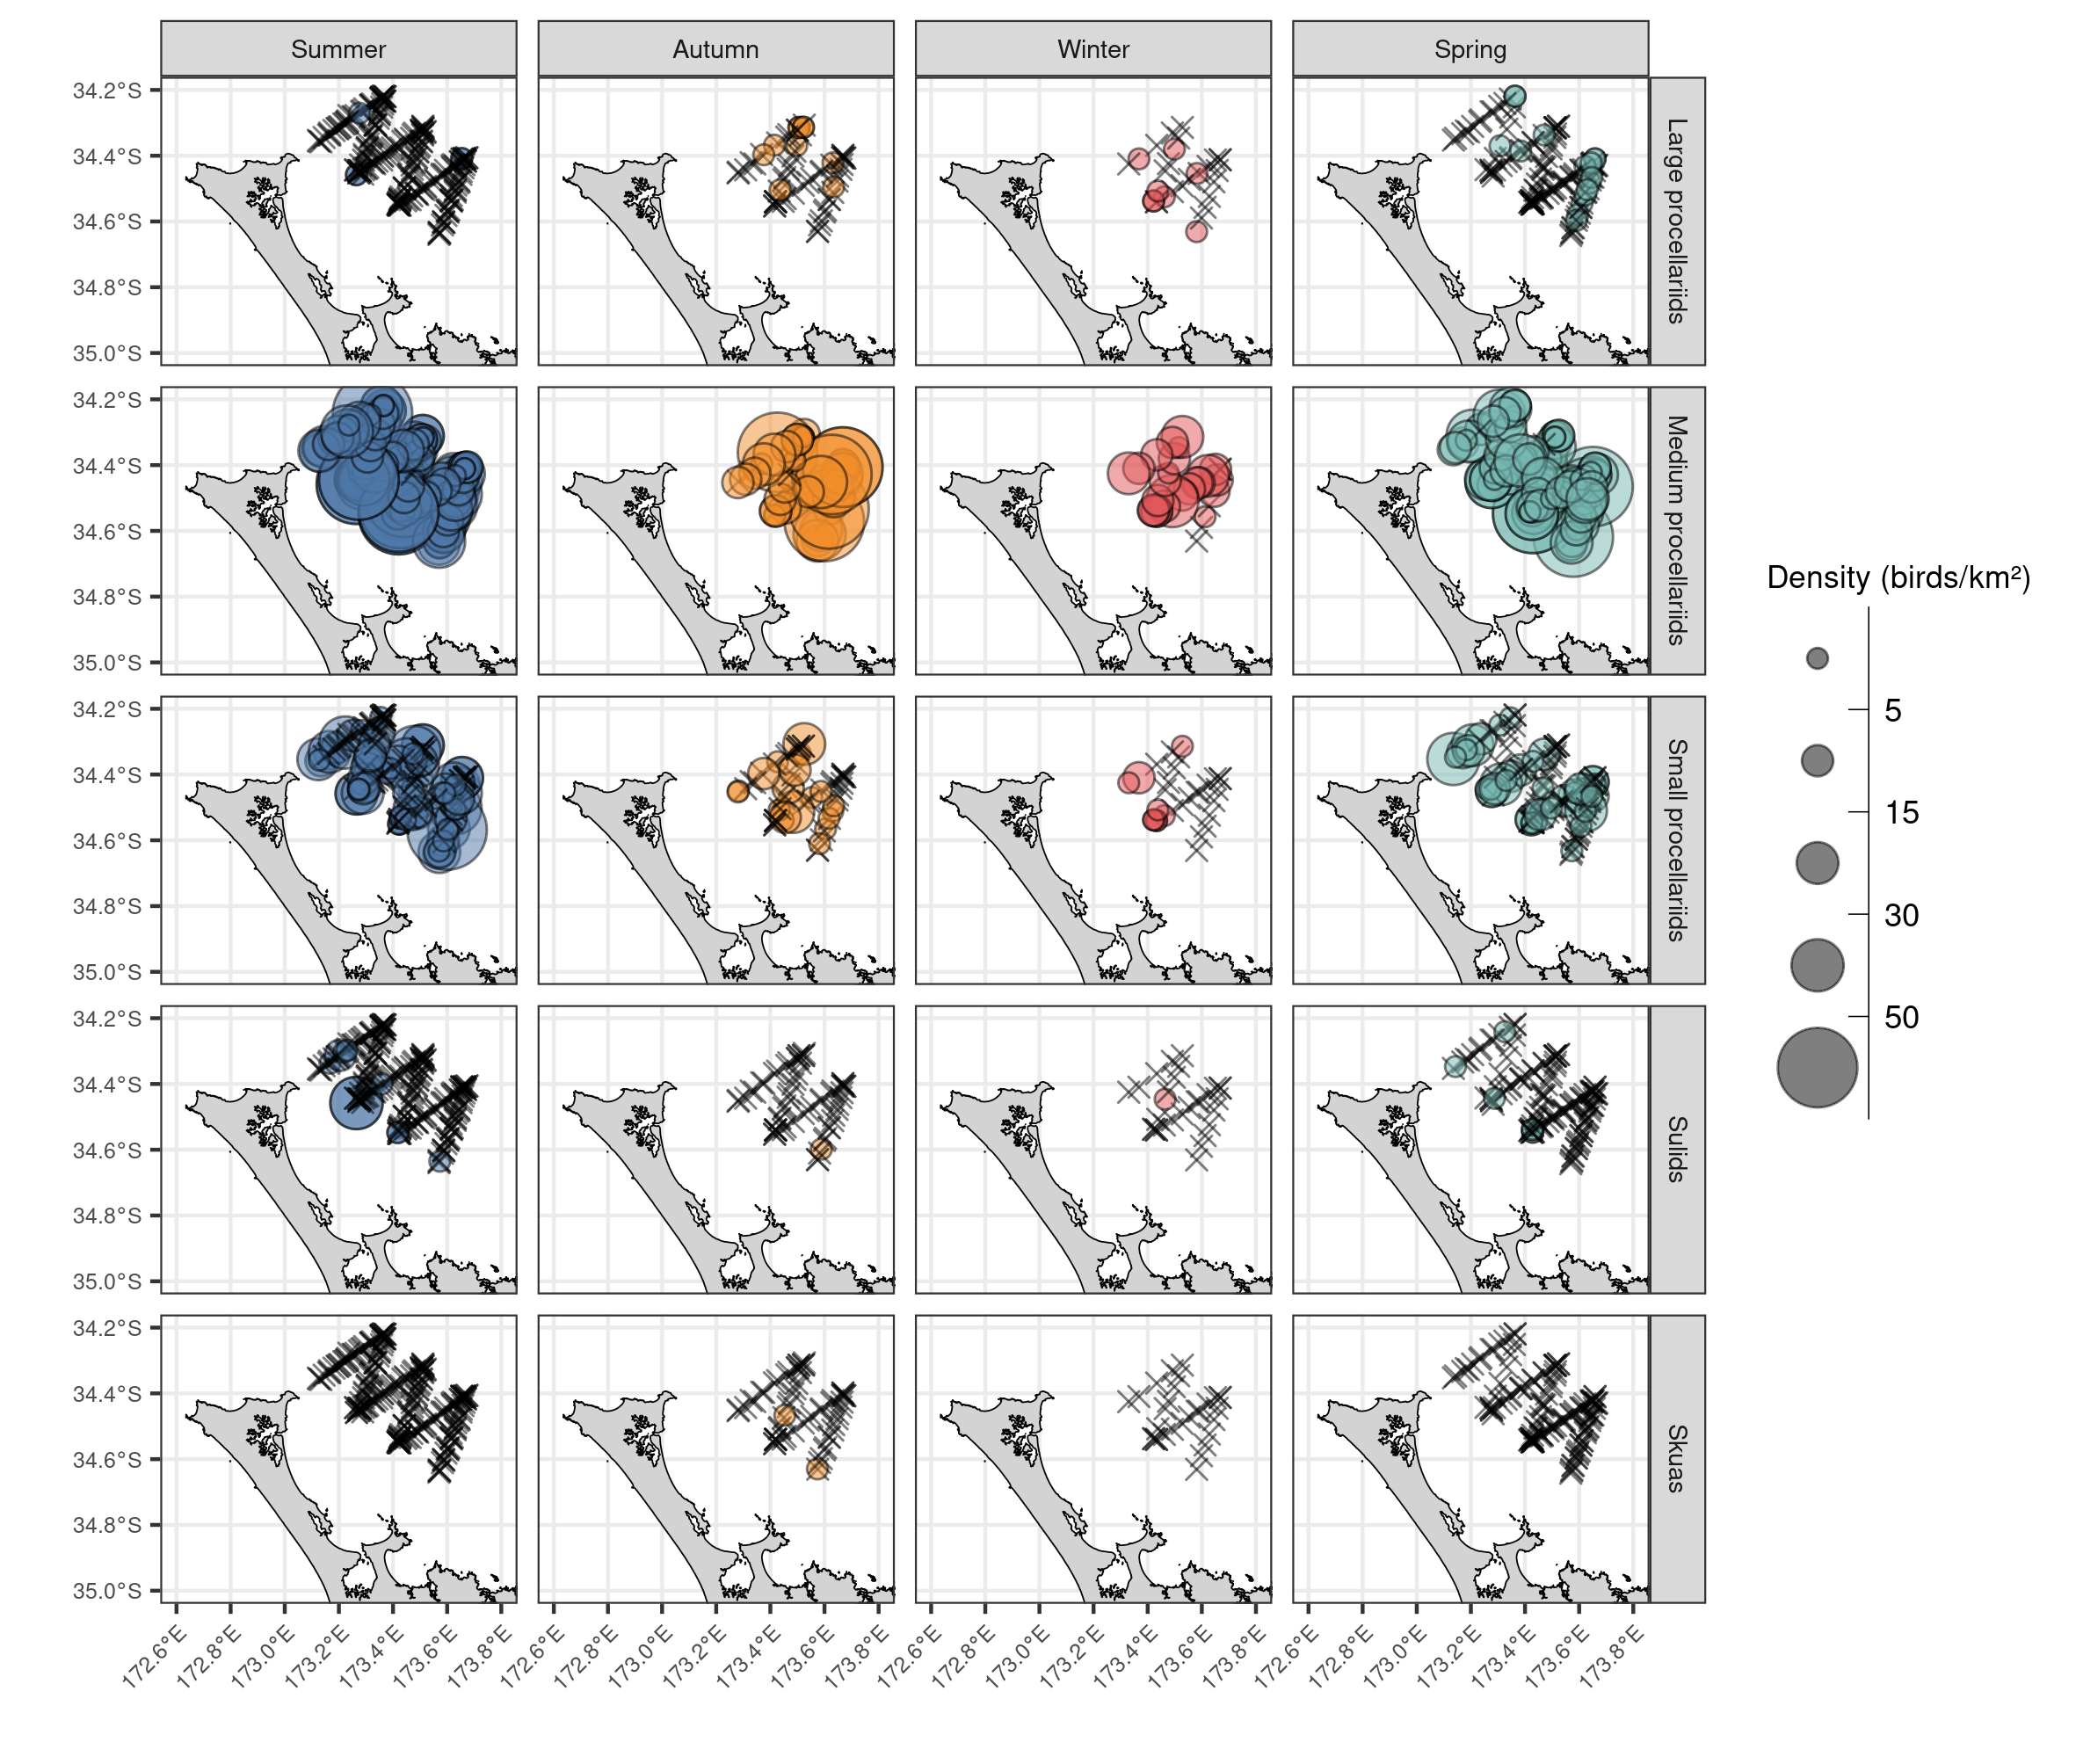
\includegraphics[width=1\linewidth]{map_grps-density_by_season.png}
\caption{Spatial representation of densities (birds/km$^2$) of seabird feeding guilds off Northland, Aotearoa/New Zealand, 2019--2024, for each season. Crosses represent 10-min counts with no record of any particular group.}
\label{fig:map-densities-farout}
\end{figure}

\begin{figure}[H]
\centering
\includegraphics[height=0.85\textheight]{violin_season_sprich-nbirds-density-biomass-by-transect.pdf} 
\caption{Violin plots summarising species richness (A), number of individuals (B), densities (birds/km$^2$; C) and biomass (kg/km$^2$; D) of seabirds off Northland, Aotearoa/New Zealand, 2019--2024, for each season. The values are summarised at the transect level; the number of transects is shown at the top of panel A. The black dot and lines represent the geometric mean and standard deviation, respectively; in panel B there are no apparent lines due to scale (standard deviations were \emph{c}. 2 for all seasons).}
\label{fig:violins-patchwork-farout}
\end{figure}

The surface oceanographic conditions exhibited low variability within each voyage (Supplementary Material Figures S2, S3). However, the TDR profiles revealed seasonal patterns in the vertical structure of the water column. Spring voyages had shallower MLDs, whereas autumn had deeper MLD following summer warming. Voyage 8 was undertaken in late May, closer to winter conditions, and showed a shallower MLD likely due to more frequent storms at this time of the year (Figure \ref{fig:tdr-profiles-farout}). Both spring voyages also recorded stratified subsurface SST structures, while in summer and autumn, the subsurface conditions were more homogeneous to 50 m (Figure \ref{fig:tdr-profiles-farout}).

\vspace{2.1cm}

\begin{figure}[H]
\centering
\includegraphics[width=1\linewidth]{TDR-profiles.pdf}
\caption{Interpolated temperature-at-depth recorder (TDR) profiles (x-axis) for five voyages off Northland, Aotearoa/New Zealand. The mixed layer depth (MLD) is shown as a cyan line; thin white lines represent isotherms at 0.5°C intervals.}
\label{fig:tdr-profiles-farout}
\end{figure}

Descriptive frequencies of occurrence and relative abundances showed a clear seasonal pattern of seabird species' presence and their numeric contribution to the assemblage (Supplementary Material Table S2). The most frequently-observed species during summer were Buller's shearwater (\emph{Ardenna bulleri}; 67.8\%), black petrel (\emph{Procellaria parkinsoni}; 60.6\%), white-faced storm petrel (\emph{Pelagodroma marina}; 39.9\%) and Cook's/Pycroft's petrel (\emph{Pterodroma cookii/pycrofti}; 34.1\%). In autumn, grey-faced petrels (\emph{Pterodroma macroptera}; 60.9\%), Buller's shearwater (29.7\%), fairy prion (\emph{Pachyptila turtur}; 21.9\%) and black petrels (20.3\%) were most frequently observed, and grey-faced petrels (63.3\%), fairy prions (30\%) and fluttering shearwaters (\emph{Puffinus gavia}; 23.3\%) in winter. In spring, flesh-footed shearwater (\emph{A. carneipes}; 49.6\%), Cook's/Pycroft's petrel (48\%), Buller's shearwater (41.7\%), grey-faced petrel (33\%) and white-faced storm petrel (28.4\%) were the most frequently observed species. Together, these species comprised 87.9\%, 89.5\%, 79\% and 78.1\% of the relative abundances for summer, autumn, winter and spring, respectively. The observed pattern of seabird species occurrences was consistent with their breeding cycles, i.e.,~species were mostly recorded during their breeding periods, then in low(er) numbers (or absent) when individuals were dispersing more widely or migrating, outside their breeding periods (Supplementary Material Table S1).

At the assemblage level, the best null model retained one latent variable (Supplementary Material Table S3) and showed no evidence of lack of fit (Supplementary Material Figure S4). The observations appeared to cluster better when coded by season rather than by SST or CHL (Figure \ref{fig:ordination-null-gllvm-farout}A vs \ref{fig:ordination-null-gllvm-farout}B, C). During summer, there was a cluster of observations for high CHL values although it largely overlaps with low values (Figure \ref{fig:ordination-null-gllvm-farout}C). Nonetheless, SST and CHL did not seem to explain the variation in the data for any season. The model including predictors retained only season as a predictor and zero latent variables (Supplementary Material Table S3), indicating that most of the variation in the data was explained by season alone. Residual plots revealed no lack of fit (Supplementary Material Figure S5). The coefficient plots show the seasonal effects on species relative numbers (Figure \ref{fig:coefplot-gllvm-farout}). Several species had their confidence interval estimated as large numbers (\textgreater100; Supplementary Material Figure S6), probably due to the relatively low sample size for those species within seasons. Nonetheless, these results align well with the descriptive frequencies (Supplementary Material Table S2).

\begin{figure}[H]
\centering
\includegraphics[height=0.9\textheight]{gllvm_null_lv1_biplot_tiled-A-B-C.pdf} 
\caption{Ordination plots based on the best null generalised linear latent variable model using counts of seabirds off Northland, Aotearoa/New Zealand, 2019--2024. Observations are colour-coded by season (A), sea surface temperature (SST; B) and chlorophyll-\emph{a} concentration (CHL-a; C). Panel (A) has a density plot on top and panels (B) and (C) are split by seasons to ease visualization.}
\label{fig:ordination-null-gllvm-farout}
\end{figure}

\begin{figure}[H]
\centering
\includegraphics[width=1\linewidth]{gllvm_pred_lv0_coefplot-season_xlim-adjusted.pdf} 
\caption{Coefficient plot based on the best generalised linear latent variable model including predictor using counts of seabirds off Northland, Aotearoa/New Zealand, 2019--2024. The effects of season are shown for each species relative to summer (specified as the intercept). Crosses represent the mean estimated coefficient and horizontal lines their confidence interval; black symbols represent estimates that are significant (do not include zero in their confidence interval). Supplementary Material Figure S6 shows the original coefficient plot without adjusting the limits of the x-axis. See Supplementary Material Table S1 for Te Reo M\={a}ori and scientific names.}
\label{fig:coefplot-gllvm-farout}
\end{figure}

The seasonal species co-occurrence patterns are shown by the residual correlation matrix of the null model. Species observed in spring/summer had high positive correlations, such as Buller's and flesh-footed shearwaters, white-faced storm petrels and black petrels. In contrast, winter species such as grey-faced petrels had higher positive correlations with fairy prions and black-browed albatrosses (\emph{Thalassarche melanophris}) (Figure \ref{fig:co-occurrence-farout}A). The residual correlations among species from the model including season as predictor (as per the best model) were retrieved but retaining one latent variable: the resulting correlation matrix showed no (or negligible) correlation among species, reinforcing that there was no need for latent variables and the role of the season in explaining most of the variability of the data (Figure \ref{fig:co-occurrence-farout}B).

\begin{landscape}

\begin{figure}[H]
\centering
\includegraphics[width=1\linewidth]{gllvm_co-occurrence_residual-correlation-matrices.pdf} 
\caption{Correlation matrix showing species co-occurrence patterns based on generalised linear latent variable models. On the left (A), the correlation matrix is based on the best `null' model; on the right (B), the correlation matrix is based on a model with one latent variable including `season' as a predictor. See Supplementary Material Table S1 for Te Reo M\={a}ori and scientific names.}
\label{fig:co-occurrence-farout}
\end{figure}

\end{landscape}

The biomass plots revealed a very strong contribution from medium procellariids, which made up more than 65\% of the total estimated biomass in all seasons (Figure \ref{fig:biomass-farout}). Larger procellariids clearly showed a seasonal pulse, with lower biomass in summer, rising in autumn, peaking in winter, and dropping their relative contribution in spring (Figure \ref{fig:biomass-farout}A, B). Sulids mainly contributed to the biomass in summer (Figure \ref{fig:biomass-farout}A, B). Skuas and small procellariids made a negligible contribution to the total biomass. The seasonal fluctuations of shearwaters and petrels largely impacted the assemblage structure, particularly Buller's and flesh-footed shearwaters and black and grey-faced petrels (Figure \ref{fig:biomass-farout}C, D). Despite the high frequency of occurrence of Cook's/Pycroft's petrels in some seasons, they made a small contribution to total biomass. Summer hosted the largest total estimated biomass (1885 kg/km$^2$), almost eight times higher than the total estimated biomass in winter (Figure \ref{fig:biomass-farout}). In autumn, the total estimated biomass decreased (683 kg/km$^2$), leading to the lowest total estimated biomass in winter (243 kg/km$^2$), which increased again in spring (1046 kg/km$^2$).

\begin{figure}[H]
\centering
\includegraphics[width=1.05\linewidth]{biomass-patchwork_otherspp.pdf} 
\caption{Seasonal total and relative estimated biomass (kg/km$^2$) of seabirds recorded off Northland, Aotearoa/New Zealand, 2019--2024, by feeding guild (A, B) and species (C, D). Note that in C and D, less representative species were grouped to highlight the main species contributions. See Supplementary Material Table S1 for Te Reo M\={a}ori and scientific names.}
\label{fig:biomass-farout}
\end{figure}

The number of species recorded seemed to plateau in summer, but with increased sample size, more species would likely be recorded during autumn and spring (Supplementary Material Figure S7A). Given its small sample size, the trends in winter are not apparent. Nonetheless, all seasons appeared to have been well sampled regarding species diversity (Supplementary Material Figure S7B). Overall, the diversity curves suggest that the dataset, although relatively small, offers valuable insights at the seasonal scale.

\section{Discussion}

This study provides the first quantitative at-sea data on seabird assemblages in the northernmost region off Aotearoa/New Zealand's mainland. Using descriptive and modelling approaches, seabird assemblages were shown to be seasonally structured according to species' phenologies. The assemblages were strongly influenced by migratory or wide-ranging dispersive species, particularly by the occurrence/absence of four migratory, medium-sized procellariids. These seasonal dynamics regulated patterns of seabird biomass in the region, which increased more than seven times in estimated total biomass between winter and summer. Data on the vertical SST structure of the water column during five voyages were obtained, supporting a better understanding of the local oceanography at the mesoscale. The results demonstrate the role of species phenologies in shaping assemblages of seabird species and their impact on total estimated biomass, which may affect the functioning and energy flux in this ecosystem.

\subsection{Seabird diversity and conservation off Northland}

A high number of species was recorded, comparable with regions of high importance for seabirds in Aotearoa/New Zealand. The wider Hauraki Gulf, a region south of the study area, is regarded as a global hotspot for seabirds, given its high number of species, individuals and endemic species \citep{karpouzi2007, gaskin2017}. \citet{stateof2021} listed 27 species of seabirds breeding there, of which 14 are procellariiforms (note they list Cook's and Pycroft's petrel separately). From those species, all but the little shearwater (\emph{Puffinus assimilis}) were recorded in this study. Between the study area and the Hauraki Gulf, \citet{brough2025} recorded 20 species of seabirds (`Cook's/Pycroft's petrel' pooled) during line transect surveys off the coast of Bream Bay (Whang\={a}rei, at the southern limit of Northland). Their surveys were closer to shore (\textless30 km), and thus, they also recorded typical coastal species such as terns \emph{Sterna} spp. and gulls \emph{Chroicocephalus} spp. Little shearwater and Buller's and grey-headed albatrosses (\emph{Thalassarche bulleri} and \emph{T. chrysostoma}, respectively) were also observed in their study but not in this study. Interestingly, the most frequent species in Bream Bay are consistent with this study's results---Buller's and flesh-footed shearwater, white-faced storm petrel and Cook's/Pycroft's petrel, however grey-faced petrels were not as frequent as in our study area \citep{brough2025}. The number of species recorded off Northland during summer and spring in this study is also similar to the average seabird species richness off the Otago coast (South Island; average = 19), another known hotspot for seabirds in Aotearoa/New Zealand \citep{daudt2025}. There is little doubt that most of the expected species were recorded, and this study confirms Northland as an important region in terms of seabird species richness.

Several of the recorded species are threatened and/or are endemic to Aotearoa/New Zealand. Sixteen of 25 species (64\%) are ranked at-risk or threatened nationally \citep{robertson2021}, and 36\% (9/25) are endemic to Aotearoa/New Zealand \citep{williams2006}. Threatened and endemic species were present year-round off Northland during this study, reinforcing the relevance of the study area for seabird conservation. Notably, the recently re-discovered endemic New Zealand storm petrel (\emph{Fregetta maoriana}) was observed throughout the year. This species is classified as `nationally vulnerable' (under the threatened category) and `critically endangered' internationally \citep{robertson2021}, with a total population size estimated at about 1600 individuals \citep{rayner2020}. At-sea captures suggest that individuals stay close to their colony during summer in the Hauraki Gulf \citep{rayner2013, rayner2020}. However, there are no comprehensive studies on their year-round distribution. The relatively higher numbers of New Zealand storm petrels recorded during autumn in this study may indicate that some individuals disperse to Northland, potentially the females, while in their pre-laying exodus \citep{rayner2013}. Due to the high prevalence of New Zealand storm petrels off Northland, it was believed that another colony could exist in the region; however, genomic analyses support the existence of a single breeding colony in the Hauraki Gulf \citep{correll2024}.

Seabird assemblages were primarily composed of oceanic species, of which 22 of 25 were procellariiforms (albatrosses and petrels). In a global analysis of procellariform diversity, Northland was featured in the top 10 regions in the world regarding species richness and endemism for both breeding and foraging species, including the grid where the authors recorded the highest number of species \citep{chown1998}. Seabirds are the most threatened bird group \citep{dias2019}, particularly albatrosses and petrels. At sea, the three main threats to procellariiforms are light pollution, bycatch and climate change (including extreme weather events) \citep{phillips2016, rodriguez2019}.

Commercial and fishing vessel deck lights attract seabirds, causing light-induced collisions \citep{black2005, merkel2011}. Northland is Aotearoa/New Zealand's commercial shipping entrance from the north, and a shipping lane goes through the study area \citep{lundquist2025}. Commercial fishing also operates in the area, potentially adding to the problem of seabird-vessel strikes \citep{ryan2021}. Moreover, vessel lights can reduce colony attendance in seabirds \citep{austad2023}, which may be particularly relevant to grey-faced petrels breeding at the cliffs of the Otou/North Cape during winter. In parallel, ship traffic can also increase the risk of birds getting oiled \citep{renner2015, wagner2023}. Significant bycatch rates of shearwaters and petrels have been consistently recorded off Northland, where the most impacted species are black and grey-faced petrels and flesh-footed shearwaters \citep{abraham2020}. Not surprisingly, these species were among the most recorded in this study. The black petrel, in particular, is considered threatened, with a `nationally vulnerable' status and globally vulnerable \citep{robertson2021}. Given these species' occurrence and relative abundance patterns, as described in this study, the reported bycatch illustrates that it is an issue throughout the year off Northland.

Finally, although SSTs off Northland appear to be changing at lower rates compared to most of Aotearoa/New Zealand \citep{sutton2019}, marine heatwaves (MHW) have been increasing in frequency, duration and intensity \citep{montie2024}. The impacts of MHW on seabird populations are not yet fully understood. Nonetheless, seabirds will need to adapt to thrive, and their adaptive capacity may depend on their behavioural plasticity and life history strategies \citep{woehler2024}. Northland will likely experience the first consequences of the global phenomenon of tropicalisation within Aotearoa/New Zealand \citep{zarzyczny2024}. Tropical and subtropical fish species historically rare in Aotearoa/New Zealand are occurring more frequently, especially in the north and northeast regions \citep{middleton2023}. Given seabirds track SST conditions, species occurrence in the region could be used as a surrogate to anticipate broader environmental changes, as documented off the Otago coast \citep{daudt2025}.

\subsection{The ecological effects of seasons on the assemblage structure and biomass}

The assemblage of oceanic seabird species off Northland may have a unique characterising features, being primarily driven by a temporal mechanism linked to species' phenologies. Seasonal seabird assemblages have been documented elsewhere, and migratory species often modify a resident assemblage upon arrival/departure \citep{renner2008, hunt2014, simon2024}. In Aotearoa/New Zealand, a similar pattern to those reported in the present study was also found off the southeast coast of the South Island \citep{daudt2025} and off the east coast of the North Island \citep{vooren1972}, where a group of resident species were frequent throughout the year but the assemblage structure was strongly influenced by migratory and dispersive species, including by locally breeding species. However, the assemblage described in this study shows that most species are wide-ranging dispersive or migrants. Therefore, the assemblage seems entirely dynamic at the seasonal scale, without a core group of `resident' species. In seabird assemblages, resident species are commonly coastal species breeding locally (e.g.,~terns, gulls) or those that do not disperse widely (e.g.,~boobies). Since the surveys only occurred in oceanic waters, coastal species were not detected. Together, the predictability and stability of the phenologies of seabird species \citep{keogan2018}, that the selected model retained only season as a predictor, and the lack of spatial patterns at the mesoscale, suggest that time alone may be the mechanism regulating the temporal diversity patterns in this assemblage \citep[see][]{tonkin2017}.

Four migratory species and their seasonal occurrence patterns strongly influenced biomass estimates. Migratory seabird species have also considerably shaped biomass patterns in other temperate regions, such as in the Aleutian Archipelago \citep{renner2008} and the Gulf of Alaska \citep{hunt2005}. Conversely, in Prydz Bay, Antarctica, \citet{woehler1997} noted that about two-thirds of the biomass was from residents during summer. Interestingly, in that study, the relationship between abundance and biomass of resident and non-resident (mostly wide-ranging) species were negatively correlated \citep{woehler1997}. The migratory black petrel and Buller's shearwater (summer), grey-faced petrel and Buller's shearwater (autumn), grey-faced petrel (winter), and flesh-footed and Buller's shearwaters and black and grey-faced petrels (spring) contributed up to and often exceeding 50\% of the total estimated biomass in each season during this study. The temporal segregation mediated by their phenologies seems to be the key to supporting their coexistence in the study area \citep{rudolf2019}. In addition, given that their relative contribution to the estimated biomass was similar within seasons and that they share ecological traits \citep{tavares2019}, these species may play a similar role in ecosystem functioning.

The total estimated biomass of seabirds varied strongly among seasons. Biomass can be used as a proxy for understanding ecosystem energy flux and quantifying biodiversity function \citep{barnes2018, jochum2021, kokubun2025}. In addition to consuming resources as predators, seabirds also redistribute essential nutrients (e.g., nitrogen, iron) in the system through their excretion (guano) \citep{wing2014, doughty2016, steibl2024}. These nutrients constrain primary productivity in low concentrations \citep{boyd2004, moore2013}. In this study, the almost eight-fold increase in biomass during summer may therefore act similarly to a `resource pulse' \citep[e.g.,][]{yang2008} regarding nutrient recycling at the seasonal scale. In the North Atlantic Ocean, recent work has demonstrated the impact of seabird guano on summer productivity \citep{browning2023}. Medium-sized petrels dominate the assemblage of seabird species using that region in terms of biomass \citep{wakefield2021}, similar to this study's results. Thus, the summer assemblage of seabirds off Northland and their high estimated biomass may play an important ecosystem role in making essential nutrients available, increasing primary productivity locally, and possibly sustaining regional fisheries.

The seasonal variation in the vertical structure of the temperature in the water column did not appear to be related to the predominant foraging method of the seabird assemblage (pursuit-diving and surface-seizing). Given that thermal stratification regulates the depth at which seabird prey concentrate \cite[e.g.,][]{davoren2006, cox2013}, it directly influences prey availability and, consequently, the distribution of seabirds \citep{scott2010, cox2018, serratosa2020}. Deeper dives are usually required in mixed, more homogeneous water structures than stratified, heterogeneous structures \citep{takahashi2008, meyer2020}, which may limit species that cannot dive deep. Thus, changes in the vertical structure of the water column may correlate with changes in feeding guilds. The TDR profiles documented seasonal differences in the water column off Northland, although the MLD was relatively shallow (\textasciitilde20 m depth) in all but the mid-autumn voyage (\textasciitilde40 m depth). The seabird assemblages were numerically dominated by four procellariids that use a mix of surface-seizing and pursuit-diving. Although there are limited data on diving behaviour of Buller's and flesh-footed shearwaters (pursuit-divers), shearwaters can dive more than 50 m depth \citep{taylor2008, rayner2011} and are thus more likely to adjust their foraging/diving behaviour according to their prey availability. The surface-seizing black and grey-faced petrels dive up to 10 m depth, averaging 2 to 5 m \citep{dunphy2015, bell2016}. These species, however, feed mainly on bioluminescent prey at night \citep{imber1973, imber1976}, which may buffer the consequences of a deeper MLD during autumn. Although we have not collected data on the water-column structure during winter, we expect that windy conditions lead to deeper MLD \citep{serazin2023}. Contrary to what would be expected by considering MLD depth alone, large procellariids (surface-feeders) contributed to about a third of the total estimated seabird biomass in winter. The mismatch between MLD patterns and seabird feeding guilds reinforces that, at the assemblage level, temporal patterns seem to be more important than oceanographic conditions.

\subsection{Limitations of the study}

It is acknowledged that the dataset is relatively modest in terms of sample size. Due to the survey design, not all possible species in the region were recorded. Various factors may have influenced this, but most likely, the focus on offshore waters and the limited sample size. For instance, fluttering shearwater is abundant in the region but prefers coastal waters over the shelf \citep{berg2019}. Thus, their occurrence in the dataset may not reflect their regional presence in this area. Uncommon species passing through the area during `off effort' periods were opportunistically recorded (e.g.,~brown booby [\emph{Sula leucogaster}] and grey ternlet [\emph{Procelsterna cerulea}]). Nonetheless, as the probability of detecting species relates to their relative abundance \citep{mccarthy2013}, these species seem naturally infrequent in the area. Additionally, some voyages were only two days long, which may have reduced the chances of recording some species. However, the coverage-based diversity curves suggested that the dataset seems to have captured most of the relevant species at the seasonal level.

The sampling design could have also limited the ability to detect spatial and temporal relationships between species and environmental parameters. The study area is relatively small compared to seabird movements. For instance, Buller's shearwaters may commute daily from the Poor Knights Islands to feed off Northland (roughly 140 km) \citep{whitehead2023}, whereas the study area is about 40 km long. \citet{whitehead2023} also showed that Buller's shearwaters are associated with higher Finite Size Lyapunov Exponent (FSLE) values in the study area. This metric indicates dynamic sub-mesoscale fronts, where seabirds forage \citep{tewkai2009, scales2014mesoscale}. Surface chlorophyll-\emph{a} fine-scale fronts have been also shown to influence seabird distributions in Aotearoa/New Zealand \citep{lheriau2025}. Thus, using finer temporal and spatial scale environmental variables, or additional environmental variables along with potential lagged relationships, could have helped understand the relationships between species and their environment. Nonetheless, the analysis concentrated on the assemblage level rather than individual species, so we are confident that the results captured what drives the multi-species occurrence pattern, i.e.,~seasons and species phenologies.

\section{Conclusions}

This study provides evidence of an oceanic seabird assemblage driven by seasonality. Most species recorded are migratory or wide-ranging dispersive, and several are nationally or globally threatened. The northeast of Aotearoa/New Zealand is therefore a region of paramount importance for seabird conservation. Furthermore, given the study area is in the northernmost region of Aotearoa New Zealand, it is likely to be the first region to experience the consequences of global warming. These are the first at-sea, systematic survey data for this region and provide a baseline against which to measure changes. Therefore, continued monitoring is encouraged to better understand the importance of Northland waters to seabirds---given that several threatened species use the area---and to assess tropicalisation using \emph{in situ} data on not only seabird distributions but also on oceanographic parameters (e.g., TDR measurements).

The results also show the overwhelming influence of four species in regulating biomass patterns, which may have direct implications for ecosystem functioning (e.g.,~resource partitioning, primary productivity). The assemblage dynamics reported here may be unique to Aotearoa/New Zealand, where multiple seabird species and many individuals overlap at sea, particularly medium-sized procellariids. Thus, time appears to be of the essence for specious seabird assemblages living in sympatry.

\hypertarget{acknowledgements}{%
\section*{Acknowledgements}\label{acknowledgements}}
\addcontentsline{toc}{section}{Acknowledgements}

We acknowledge Ng\={a}ti Kuri as kaitiaki (guardians) of the rohe moana (territory) where this research occurred and thank them for their support. The Far Out Research Collective thanks the many volunteers and collaborators who helped during fieldwork, including Lily Kozmian-Ledward, Alice Della Penna, Momoko Burgess, Catherine Meyer, Maurice Kaprowsky, Brett Sutton, Lucy McLeod and Diana Galbraith for their help over multiple surveys. Special thanks to Geir Sveaass, whose enthusiasm and support were fundamental to keeping us comfortable and in a good mood. Thanks also to the Moana Project for providing the Mang\={o}pare sensor. NWD thanks the Department of Marine Science (University of Otago) for supporting a PhD writing retreat, during which most of this manuscript was drafted. NWD was supported by a Doctoral scholarship from the University of Otago, Aotearoa/New Zealand; LB is a research fellow of the Conselho Nacional de Desenvolvimento Científico e Tecnológico (CNPq), Brazil (Grant No. 310145/2022-8).

% \hypertarget{references}{%
% \section*{References}\label{references}}

\bibliographystyle{elsarticle-harv}
\bibliography{mybibfile.bib}

\newpage

\hypertarget{authors-contribution-credit}{%
\section*{Authors' contribution (CRediT)}\label{authors-contribution-credit}}
\addcontentsline{toc}{section}{Authors' contribution (CRediT)}

\textbf{Nicholas W. Daudt:} Conceptualization; Methodology; Investigation; Data Curation; Software; Formal analysis; Visualization; Writing - Original Draft. \textbf{Marta Guerra:} Conceptualization; Resources; Investigation; Writing - Review \& Editing. \textbf{Tom Brough:} Conceptualization; Resources; Investigation; Writing - Review \& Editing. \textbf{Sarah L. Dwyer:} Conceptualization; Resources; Investigation; Writing - Review \& Editing. \textbf{Jochen R. Zaeschmar:} Conceptualization; Resources; Investigation; Writing - Review \& Editing. \textbf{Matthew R. Schofield:} Writing - Review \& Editing; Supervision. \textbf{Robert O. Smith:} Writing - Review \& Editing; Supervision. \textbf{Leandro Bugoni:} Writing - Review \& Editing; Supervision. \textbf{Eric J. Woehler:} Conceptualization; Writing - Review \& Editing; Supervision. \textbf{William J. Rayment:} Conceptualization; Investigation; Writing - Review \& Editing; Supervision.

\hypertarget{orcid}{%
\section*{ORCID}\label{orcid}}
\addcontentsline{toc}{section}{ORCID}

Nicholas W. Daudt -- \url{https://orcid.org/0000-0001-8211-8771}

Marta Guerra -- \url{https://orcid.org/0000-0002-0244-361X}

Tom Brough -- \url{https://orcid.org/0000-0003-1835-0490}

Sarah L. Dwyer -- \url{https://orcid.org/0000-0002-9244-8114}

Jochen R. Zaeschmar -- \url{https://orcid.org/0000-0002-6978-0995}

Matthew R. Schofield -- \url{https://orcid.org/0000-0003-1481-2766}

Robert O. Smith -- \url{https://orcid.org/0000-0001-5931-3843}

Eric J. Woehler -- \url{https://orcid.org/0000-0002-1125-0748}

Leandro Bugoni -- \url{https://orcid.org/0000-0003-0689-7026}

William J. Rayment -- \url{https://orcid.org/0000-0001-9558-5109}


\hypertarget{data-availability-statement}{%
\section*{Data Availability Statement}\label{data-availability-statement}}
\addcontentsline{toc}{section}{Data Availability Statement}

The data were collected on the rohe moana (territory) of the local iwi Ng\={a}ti Kuri. Following the CARE principles, we respect the wish of the local indigenous people not to make the raw data publicly available. For the same reasons, species-specific distribution maps were not, and will not be, shown without their previous consent. If you are interested in the raw data, please contact the Far Out Ocean Research Collective (\url{https://www.farout.org.nz/}). The analysis code is available for transparency at \url{https://github.com/nwdaudt/far-out_seabirds/}, and will be archived as a hard-copy upon manuscript acceptance.

\hypertarget{conflict-of-interest-disclosure}{%
\section*{Conflict of interest disclosure}\label{conflict-of-interest-disclosure}}
\addcontentsline{toc}{section}{Conflict of interest disclosure}

The authors declare that they have no known competing financial interests or personal relationships that could have appeared to influence the work reported in this paper.

\hypertarget{funding}{%
\section*{Funding}\label{funding}}
\addcontentsline{toc}{section}{Funding}

Ecocruz Bay of Islands provided the research vessel. The University of Auckland, University of Otago and the Center for Research Excellence `Coastal People: Southern Skies' provided funds towards surveys. The Rolex Explorers Club granted research funds to TB. Canon New Zealand Ltd. provided camera gear for the Far Out Ocean Research Collective.

\end{document}
